Lorem ipsum \textbf{hello world} \textit{italtic}! $\frac12$ some inline math % convert to Lorem ipsum **hello world** *italtic*! $\frac12$ some inline math

\section{Section} 
% conver to yaml header:
% ---
% title: Section
% ---

\subsection{Subsection} % convert to ## Subsection

\hyperref[sec:name]{Link to section} % convert to [FIXME](./name-of-section)
\hyperref[subsec:name]{Link to section} % convert to [FIXME](#name-of-section)
% Keep FIXME text. 

\[1+2=3\] % convert to:
% ```math
% 1+2=3
% ```

\begin{align*}
    a & = 1 + 2 \\
    a & = 3 \\
\end{align*} % convert to:
% ```math
% \begin{align*}
%     a & = 1 + 2 \\
%     a & = 3 \\
% \end{align*}

\begin{minipage}{0.5\textwidth}
Hello world
\end{minipage}
\begin{minipage}{0.5\textwidth}
Hello world
\end{minipage} 
% Use the component <HLayout split={[w, w, ...]}>...</HLayout> when converting a number of minipages that take up a width. Put the contents of each minipage into a <div> element inside the HLayout component. Split defines the width style for each child div.
% The above would be converted to:
% <HLayout split={["50%", "50%"]}> <div> Hello world </div> <div> Hello world </div> </HLayout>

\begin{definition}
{Title of definition}
Hello world
\tcblower
Hello world 2
\end{definition}
% <Block title="Title of definition" variant="primary"> Hello world <BlockSep /> Hello world 2 </Block>

\begin{theorem}
{Title of theorem}
Hello world
\end{theorem}
% <Block title="Title of definition" variant="secondary"> Hello world </Block>

\begin{knBox}
{Title of knBox}
Hello world
\end{knBox}
% <Block title="Title of definition" variant="knowledge"> Hello world </Block>

\begin{example}
{Title of example}
Hello world
\end{example}
% <Block title="Title of definition" variant="example"> Hello world </Block>

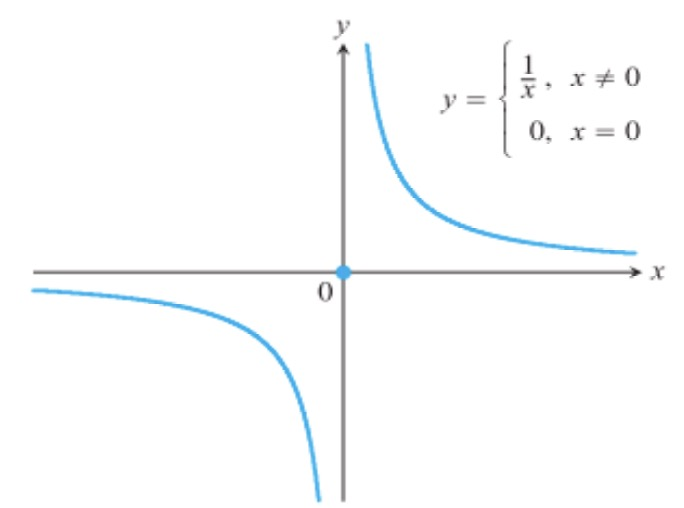
\includegraphics[width=\textwidth]{img/lim3.jpg} % convert to ![Image caption](./img/lim3.jpg)

Other environments like itemize, enumerate, etc. should be converted to markdown equivalents.
Spacing like \hfill and \vfill should be removed, as well as \label commands.
Tables should be converted using markdown tables.